%---------------------------------------------------------------------------------------
%	PAQUETES Y CONFIGURACIÓN DEL DOCUMENTO
%----------------------------------------------------------------------------------------

%%% Configuración del papel.
\documentclass[12pt]{article} 
\usepackage[utf8]{inputenc}
\usepackage[catalan]{babel}
\usepackage{blindtext}
\usepackage{graphicx} 
\usepackage[margin=3cm]{geometry}
\usepackage{subcaption}
\usepackage{listings}
\usepackage{caption}
\usepackage{hyperref}
\usepackage{url}

\newcommand{\horrule}[1]{\rule{\linewidth}{#1}} % Create horizontal rule command with 1 argument of height

\title{
  \normalfont \normalsize 
  \textsc{FIB: Probabilitat i Estadística} \\ [25pt] 
  \horrule{0.5pt} \\[0.4cm] % Thin top horizontal rule
  \huge Quina shell és la més ràpida? \\ % The assignment title
  \horrule{2pt} \\[0.5cm] % Thick bottom horizontal rule
}

\author{Rubén Catalán, Ismael El Basli i Muhammad Yasin Khokhar}
\usepackage{xcolor}

\definecolor{codegreen}{rgb}{0,0.6,0}
\definecolor{codegray}{rgb}{0.5,0.5,0.5}
\definecolor{codepurple}{rgb}{0.58,0,0.82}
\definecolor{backcolour}{rgb}{0.95,0.95,0.92}
\lstdefinestyle{mystyle}{
    backgroundcolor=\color{backcolour},   
    commentstyle=\color{codegreen},
    keywordstyle=\color{magenta},
    numberstyle=\tiny\color{codegray},
    stringstyle=\color{codepurple},
    basicstyle=\ttfamily\footnotesize,
    breakatwhitespace=false,         
    breaklines=true,                 
    captionpos=b,                    
    keepspaces=true,                 
    numbers=left,                    
    numbersep=5pt,                  
    showspaces=false,                
    showstringspaces=false,
    showtabs=false,                  
    tabsize=2
}
\lstset{style=mystyle}

%----------------------------------------------------------------------------------------
%	DOCUMENT
%----------------------------------------------------------------------------------------


\begin{document}
\maketitle % Escriu el títol

\newpage
\section*{RESUM}
\subsection*{Objectius}
El principal objectiu del treball es veure, donades 8 shells de UNIX concretes, poder determinar quina de totes
és la més ràpida. Per altra banda també volem veure si hi ha algun tipus de relació lineal entre el temps s'usuari
i el de sistema. Les hipòtesis que plantegem en relació a aquests objectius són que realment les shells són igual
de ràpides, ja que sinó tothom utilitzaria la mateixa shell, i que no hi ha relació entre el temps d'usuari i el de sistema.
Com a objectiu secundari, pretenim millorar la nostra habilitat usant R i aprendre \LaTeX, amb el que està fet aquest informe.
\subsection*{Mètodes}
Per a la recollida de dades, per cadascuna de les 8 shells que s'estudien al treball, hem realitzat 8 execucions d'una partida
de l'assignatura EDA de la FIB i 8 d'un programa en bash script que ordena un vector de 10000 elements. Ens hem assegurat que hi 
hagi igualtat de condicions carregant el portàtil durant les execucions i borrant la memòria cache entre execucions. Les proves
es realitzen en un computar amb arquitectura AMD: Ryzen 5 3500U a 2.1GHz, 8GB de RAM i amb sistema operatiu Debian GNU/Linux 11 bullseye.

\subsection*{Resultats i discussió}
Els resultats obtinguts indiquen que res s'oposa a assumir que les shells són igual de ràpides, ja que l'hipòtesi nul·la corresponent
a pensar que les mitjanes de temps d'execució són iguals implica un p-value gran i superior al risc, igual que en el cas de l'estudi de la relació entre el temps
d'usuari i el de sistema, on l'hipòtesi nul·la era que la pendent de la recta era 0, que no hi havia rel·lació. Per tant, és versemblant 
pensar que les shells són igual de ràpides i que el temps de sistema no justifica per res la variabilitat del temps d'usuari, ja que no
hi ha cab tipus de relació lineal.

\newpage
\section{Introducció}
Com a estudiants d'enginyeria informàtica, estem molt acostumats a treballar dintre d'una shell,
que es tracta de l'intèrpret de comandes, un programa que proveeix una interfície d'usuari
per accedir als serveis del sistema operatiu. La qüestió és que no només n'existeix una, sinó
que hi ha una gran variabilitat en quant a opcions possibles. Això ens va fer preguntar-nos si 
totes són igual de ràpides o realment hi ha diferències de velocitat considerables. Cal deixar clar
que contemplem només les shells de sistemes operatius basats en UNIX, com ara Linux o MacOS. Per exemple,
als laboratoris de la FIB treballem amb la \textit{tcsh} shell, mentre que la \textit{bash} shell és 
la més popular en la majoria dels sistemes Linux i, de fet, normalment és la predeterminada per 
les contes d'usuari. Llavors, amb quina shell ens quedem?


\subsection{Objectius}
\begin{enumerate}
  \item Ser capaços d'argumentar quina shell és la més ràpida de totes o si realment hi ha diferències 
    mínimes en quan a velocitat, tot en base a càlculs estadístics.
  \item Veure si hi ha certa relació lineal o no entre el temps d'usuari i el temps de sistema que s'usa
    per executar els programes que emprarem per evaluar les velocitats de les shells.
  \item Poder consolidar tot el que s'ha après a l'assignatura, aplicant-ho a tot el càlcul estadístic
    que implica aquest petit projecte.
  \item Millorar la nostra habilitat utilitzant R, un llenguatge de programació enfocat a l'anàlisi
    estadístic.
  \item Com a objectiu més secundari, que no té gaire a veure amb l'assignatura, aprendre \LaTeX, que 
    és un sistema de composició de textos orientat a la creació de documents escrits que presentin una
    alta qualitat tipogràfica, i amb el que està fet aquest document.

\end{enumerate}

En quant a aquests objectius, després d'haver reflexionat, són totalment factibles i estan a l'abast
dels nostres recursos i possibilitats, ja que simplement haurem de fer mesures del temps que triguen
certes shells entre l'inici i el final de determinats programes.
\newpage

\section{Variables}
L'estudi presenta la variable explicativa S $\equiv$ ``Tipus de shell'' i el seu univers $\Omega$ és:
\begin{itemize}
  \item \textbf{Bourne Shell} (sh): Intèrpret de comandes interactiu. Inclou característiques com 
    el llistat, lectura i protecció de fitxers, creació i eliminació de processos, etc.
  \item \textbf{Almquist shell} (ash): Escrita per Kenneth Almquist com un reemplaç del shell Bourne 
    a les versions BSD de Unix.
  \item \textbf{Bourne-Again shell} (bash): Escrita pel projecte GNU, serveix com a superconjunt 
    d’instruccions basades en l’intèrpret del que origina, Bourne.
  \item \textbf{Debian Almquist Shell} (dash): Conté menys comandes que Bash, però requereix de 
    menys llibreries. Algunes de les funcionalitats faltants són requerides per POSIX. 
  \item \textbf{Korn Shell} (ksh): A més d’intèrpret, serveix com a llenguatge de programació, 
    gràcies a les seves funcions per administrar arxius de comandes. 
  \item \textbf{Z shell} (zsh): Dissenyada per us interactiu com a subconjunt d’altres shells com 
    sh, bash, ksh, etc.
  \item \textbf{TENEX C shell} (tcsh): Shell amb un llenguatge de comandes similar a C que serveix 
    com a reemplaç de C Shell gràcies a característiques com la autocompleció de noms.
  \item \textbf{Friendly Interactive Shell} (fish): Considerada una shell “exòtica” ja que la 
    seva sintaxis no prové de cap altra shell. Pretén ser una shell “user-friendly”.
\end{itemize}
El motiu pel qual s'han escollit aquestes shells concretes de totes les que existeixen, és perquè són
les que s'usen més habitualment i, a més, són les que per opinió popular podrien arribar a ser les més 
ràpides. És evident que no és factible incloure totes les shells de UNIX, ja que ens extendriem massa
i probablement les shells que no contemplem en aquest projecte no arribarien a ser les més ràpides. Per
una banda, sis de les shells incloses (sh, ash, bash, dash, ksh, zsh) són compatibles amb Bourne Shell,
tcsh és compatible amb la shell de C i fish és una shell una mica més exòtica que hem volgut incloure
degut a que hi ha una opinió generalitzada que diu que es bastant ràpida.\\

Una altra variable explicativa en aquest estudi és P $\equiv$ ``Tipus de programa que s'executa'' i el
seu univers $\Omega$ és:
\begin{itemize}
  \item Ordenació de vectors: Es tracta d'un shell script (.sh) que utilitza un quicksort per ordenar un 
    vector desordenat de 10000 elements. Aquest vector és sempre el mateix, per evitar afavorir a alguna shell. El
    codi del programa està disponible a l'ANNEX.
  \item Partida joc EDA: Es tracta de l'execució d'una partida del joc de l'assignatura Estructures de Dades i Algoritmes
    on nosaltres hem de programar l'intel·ligència d'un jugador. Les partides s'executen amb un jugador anomenat
    PEplayer, que no fa res de forma aleatòria. A l'ANNEX hi haurà disponible un enllaç per descarregar el codi font del 
    joc i el codi de l'intel·ligència de PEPlayer.
\end{itemize}

En quant a aquesta variable explicativa, cal destacar certs aspectes. En un principi, preteníem que hi 
haguessin 4 tipus de programes diferents, els ja mostrats i dos més: comanda \textit{tree /} i un programa
de gestió de processos fet en bash script que ja teníem creat. El principal problema que ens va portar això
va ser que els temps d'execució d'aquests altres dos programes diferien bastant respecte els altres i això, juntament
amb les poques execucions per programa a cada shell, ens va portar problemes a l'hora d'assegurar la premissa
de normalitat per realitzar l'anàlisi estadístic. L'objectiu que teníem en ment era que els programes no 
impliquessin molta desviació cap a un tipus de gestió concreta per part de la shell, ja que l'objectiu principal
és intentar saber quina és la shell més ràpida en termes globals. Això és complicat, i més endevant es discutirà.


Ja passant a la variables de resposta, la primera i principal es tracta de T $\equiv$ ``Temps que triga una shell 
en executar un programa, en segons''. És evident que aquesta variable és mesurable, 
ja que disposem de diverses eines que ens permeten mesurar el temps entre l'inici i el final de 
l'execució d'un programa, que són adequades per llegir els valors en qüestió. En concret, 
l'instrument que s'usarà pel càlcul dels temps que triguen certes shells a executar determinats 
programes serà la comanda \textit{/usr/bin/time} de UNIX.

Les altres dues variables de resposta són el ``Temps d'usuari que consumeix l'execució d'un programa a una shell'' i
``Temps de sistema que consumeix l'execució d'un programa a una shell''. El valor d'aquestes també és
fàcilment obtenible amb la comanda \textit{/usr/bin/time} mencionada abans. Ens permetran veure si hi ha o no
relació entre el temps de sistema i el d'usuari, almenys en els programes que estudiarem.

\section{Pla de Recollida i procés de mostreig}
Pel que fa al nombre de dades que recollirem, seran 384. Aquesta n ve de 8 shells x 2 programes x 8 
execucions x 3 (temps total, de sistema i d'usuari) = 384. Considerem que aquest nombre de dades a 
recollir és suficient per arribar a complir els nostres objectius. Totes aquestes dades les recollirem en 
un computador amb arquitectura AMD: Ryzen 5 3500U a 2.1GHz, 8GB de RAM i amb sistema operatiu Debian GNU/Linux 11 bullseye. 
Totes les execucións es duran a terme a Kitty, que es tracta d'una de les terminals més ràpides actualment.
Un punt molt important i que, de fet, és premissa indispensable per l'anàlisi estadístic és l'aleatorietat
de les mostres. A la nostre recollida de dades ens assegurem d'això esborrant la memòria cachè abans de cada execució, 
mitjançant l'execució en mode root de la comanda "sync \& \& echo 3 \textgreater /proc/sys/vm/drop\_caches". A més,
en els programes que usem no hi ha cap aspecte aleatori que pugui afavorir a una shell en concret en algún cas. De fet,
també realitzem totes les execucions amb l'ordinador carregant-se, ja que el computador es tracta d'un portàtil, i no 
volem que el nivell de bateria afecti al rendiment, i per consegüent a les nostres mostres.

\section{Resultats}
\subsection{Temps total per cada shell}
La mitjana mostral del temps total d'execució (en segons) de cadascuna de les shells ha sigut:
\begin{itemize}
  \item sh: 3.56125
  \item ash: 3.563125
  \item bash: 3.56 
  \item dash: 3.569375
  \item ksh: 3.57125
  \item zsh: 3.536875
  \item tcsh: 3.541875
  \item fish: 3.55625
\end{itemize}

A la Figura \ref{fig:boxplot} es pot observar un boxplot del temps total a cada shell. D'esquerra a dreta: sh, ash,
bash, dash, ksh, zsh, tcsh i fish.

\begin{figure}[h!]
  \centering
  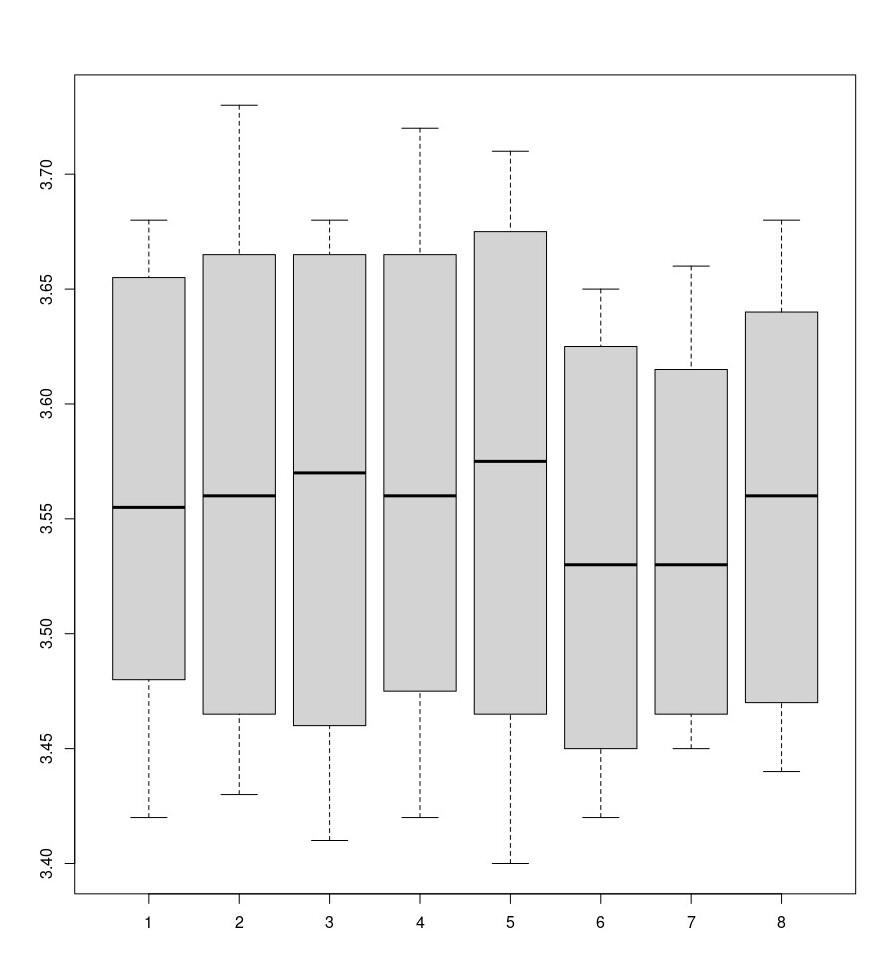
\includegraphics[width=9cm, height=7.5cm]{boxplot.jpg}
  \caption{Boxplot del temps total a cada shell}
  \label{fig:boxplot}
\end{figure} 

\newpage
Per poder comparar el paràmetre poblacional $\mu$ del temps total d'execució entre totes les shells, que són mostres independents,
podem usar el model estadístic: Y = $\mu$ + $\upsilon_{k}$ + $\epsilon$. El model contempla $\mu$ com a mitjana de referència i $\upsilon_{k}$ 
com a canvi de la mitjana del grup k.

Per poder usar aquest model hi ha certes premises. Primerament que la mostra sigui aleatòria, cosa que ja s'ha argumentat anteriorment.
A més ja es veu com no es segueix cap patró a les dades obtingudes, com es pot veure a la Figura \ref{fig:ind1}. També es requeriex 
normalitat, cosa que es compleix per totes les shells, com es pot veure a la Figura \ref{fig:norm1}. Finalment, també hi ha variabilitat 
semblant entre els grups.

\begin{figure}[h!]
  \centering
  \begin{subfigure}[b]{0.75\linewidth}
      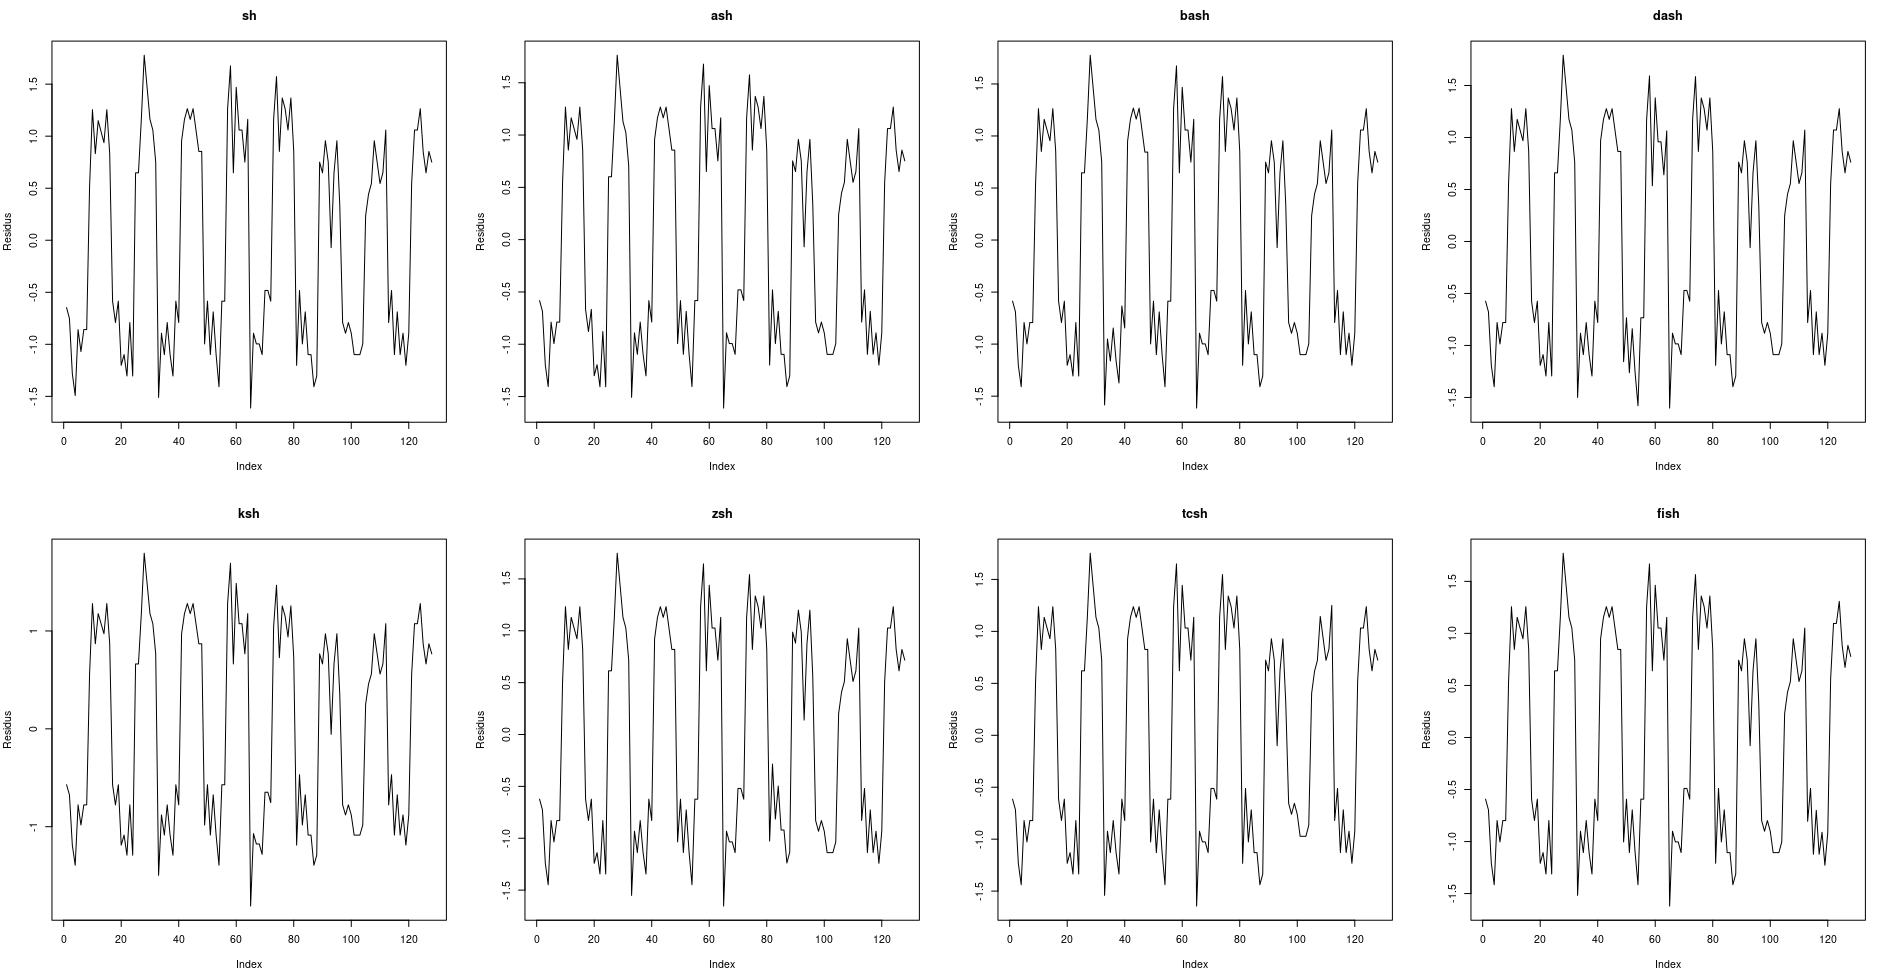
\includegraphics[width=\linewidth]{ind1.png}
      \caption{Independència}
      \label{fig:ind1}
  \end{subfigure}
  \begin{subfigure}[b]{0.75\linewidth}
    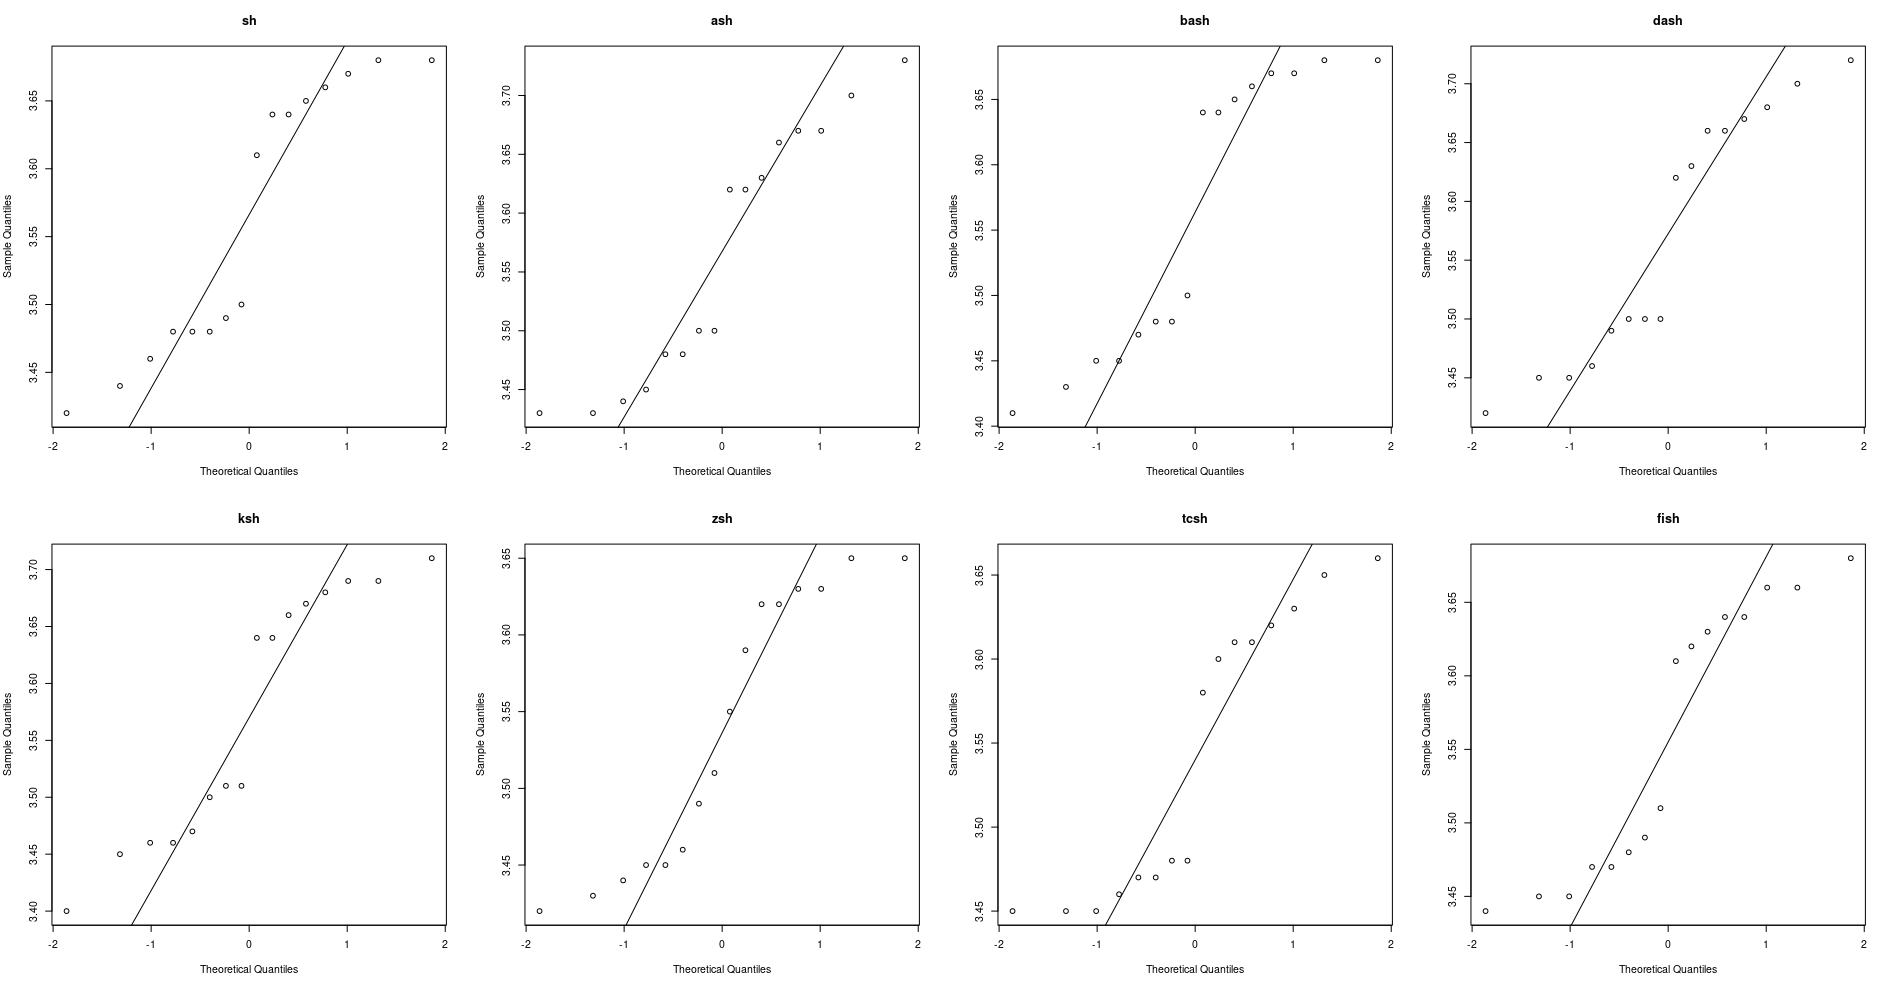
\includegraphics[width=\linewidth]{norm1.png}
    \caption{Normalitat}
    \label{fig:norm1}
  \end{subfigure}
  \caption{Premisses}
  \label{fig:prem1}
\end{figure}

Es poden arribar a apreciar dos subgrups de punts a la Figura \ref{fig:norm1}, que corresponen als temps de cadascun
dels dos programes pel testeig.
\newpage
Ara, ja demostrades les premisses del model, podem emprar la comanda lm de R per poder inferir les mitjanes de temps:
\begin{figure}[h!]
  \centering
  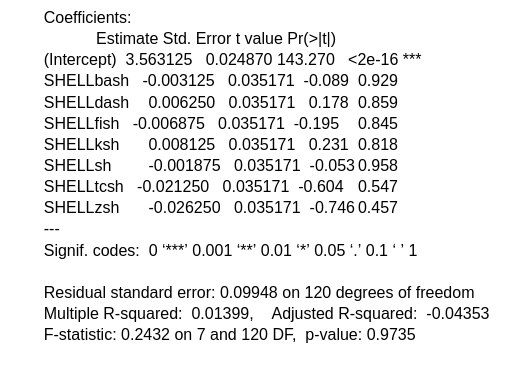
\includegraphics[width=15cm, height=8cm]{lm1.png}
  \caption{Sortida comanda lm}
  \label{fig:lm1}
\end{figure} 

A partida de la sortida de la comanda lm que es pot observar a la Figura \ref{fig:lm1}, es poden obtenir les estimacions
de les 8 $\mu$ poblacionals, en segons:
\begin{itemize}
  \item sh: 3.563125 - 0.001875 = 3.56125
  \item ash: 3.563125
  \item bash: 3.563125 - 0.003125 = 3.56
  \item dash: 3.563125 + 0.006250 = 3.569375
  \item ksh: 3.563125 + 0.008125 = 3.57125
  \item zsh: 3.563125 - 0.026250 = 3.536875
  \item tcsh: 3.563125 - 0.021250 = 3.541875
  \item fish: 3.563125 - 0.006875 = 3.55625 
\end{itemize}
\hfill \break
Per altra banda, també podem obtenir els intervals de confiança, amb un nivell de confiança del 95\%, per cadascun dels paràmetres,
mitjançant la sortida de la comanda en R confint, com es pot veure a la Figura \ref{fig:conf1}. Per altra banda, també es poden veure
els intervals de confiança de forma gràfica mitjançant la comanda emmeans de R, com es pot veure a la Figura \ref{fig:conf1i}.
\begin{figure}[h!]
  \centering
  \begin{subfigure}[b]{0.45\linewidth}
      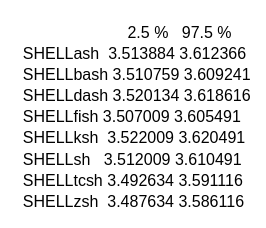
\includegraphics[width=\linewidth]{conf1.png}
      \caption{Sortida comanda confint}
      \label{fig:conf1}
  \end{subfigure}
  \begin{subfigure}[b]{0.45\linewidth}
    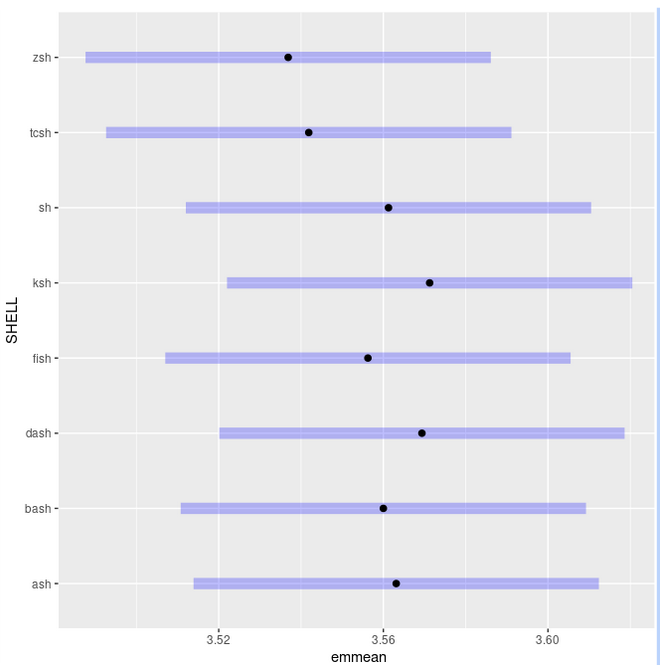
\includegraphics[width=\linewidth]{conf1i.png}
    \caption{Sortida comanda emmeans}
    \label{fig:conf1i}
  \end{subfigure}
  \caption{Intervals de confiança}
  \label{fig:ic1}
\end{figure}

Després d'haver mostrat tots els resultats es deduïble que, més enllà que una shell té una mitjana menor a les demés,
pràcticaments no hi ha diferències. Tot això es discutirà més endevant.

\subsection{Relació entre temps d'usuari i de sistema}
Per poder veure si existeix algun tipus de relació entre el temps d'usuari i el de sistema, es pot usar el model estadístic
lineal Y = $\beta_{0}$ + $\beta_{1}$X + $\epsilon$, on Y representaria el temps d'usuari i X el temps de sistema. Igual que a l'apartat
anterior, per poder usar aquest model estadístic per analitzar les nostres dades, cal demostrar certes premisses. En aquest cas
són 4: 
\begin{itemize}
  \item Mostra aleatòria
  \item Linealitat entre Y i X: Y i X s'han de poder ajustar a una recta
  \item Normalitat als residus
  \item Independència als residus: Els residus no han de seguir cap patró
  \item Homoscedasticitat als residus: Hi ha d'haver variabilitat semblant entre els grups.
\end{itemize}

Com que vàrem tenir problemes a l'hora d'assegurar aquestes premisses per poder realitzar l'estudi, ens vam veure obligats a separar l'anàlisi
per programa. 

\subsubsection{Ordenació de vectors}
Pel cas de l'ordenació de vectors, a la Figura \ref{fig:prem2}, de dalt a baix i d'esquerra a dreta s'observa la premissa
de homoscedasticitat, normalitat dels residus, linealitat i independència . A més, l'aleatorietat de les mostres es compleix pel que s'ha 
argumentat en apartats anteriors.

\begin{figure}[h!]
  \centering
  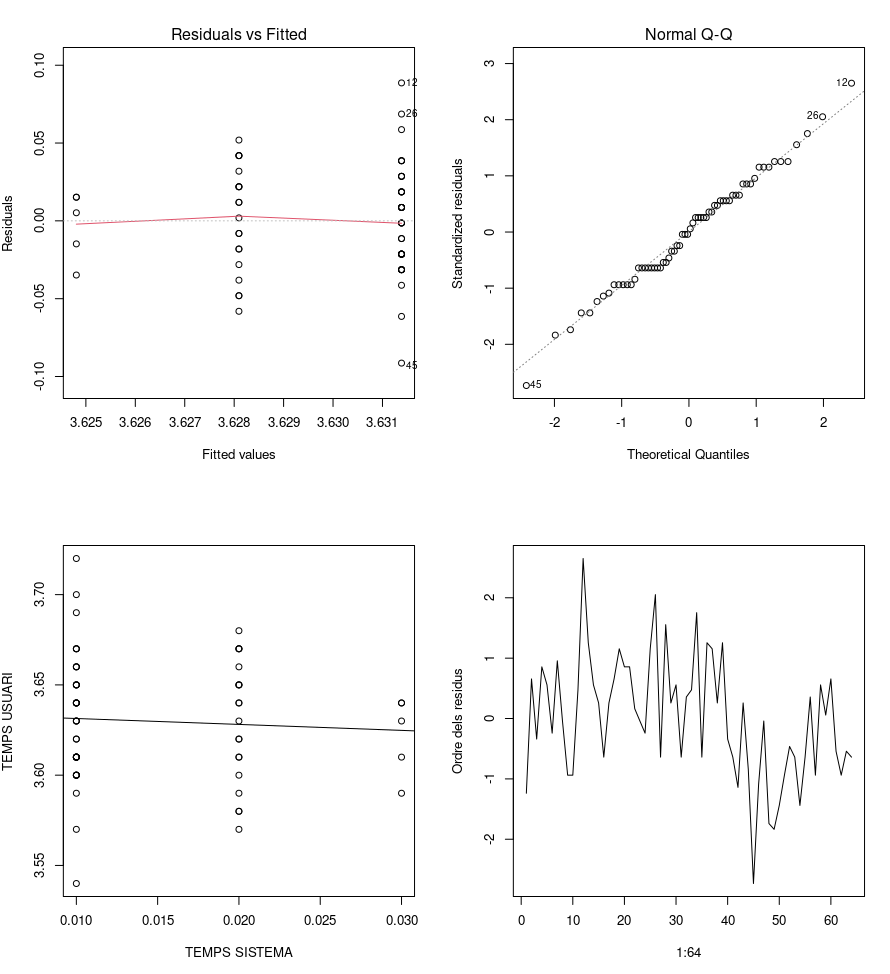
\includegraphics[width=15cm, height=10cm]{prem2.png}
  \caption{Premisses}
  \label{fig:prem2}
\end{figure} 

Tot i que són poques dades, res s'oposa a validar cap de les 4 premisses.
Ara, podem usar la comanda lm per poder veure com és la recta a la que s'ajusten el temps d'usuari i de sistema al programa d'ordenació
de vectors, per poder inferir quin tipus de relació hi ha entre ells:

\begin{figure}[h!]
  \centering
  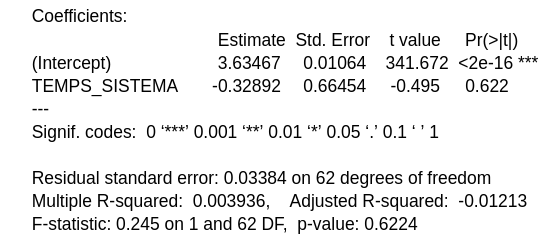
\includegraphics[width=10cm, height=6cm]{lm2.png}
  \caption{Sortida comanda lm}
  \label{fig:lm2}
\end{figure} 

A la Figura \ref{fig:lm2} es pot veure clarament com l'R-squared, que es tracta del coeficient de determinació, pren un valor molt proper
a 0, pel que X no determina per res la variació de Y. És a dir, el temps d'usuari no influeix en com varia el temps de sistema. Per aquest
motiu, no té sentit parlar de la recta que relacions ambdues variables que ens dona la comanda lm de R.

\hfill \break
\subsubsection{Partida EDA}
Pel cas de la partida d'EDA, a la Figura \ref{fig:prem3}, de dalt a baix i d'esquerra a dreta s'observa la premissa
de homoscedasticitat, normalitat dels residus, linealitat i independència . A més, l'aleatorietat de les mostres es compleix pel que s'ha 
argumentat en apartats anteriors.

\begin{figure}[h!]
  \centering
  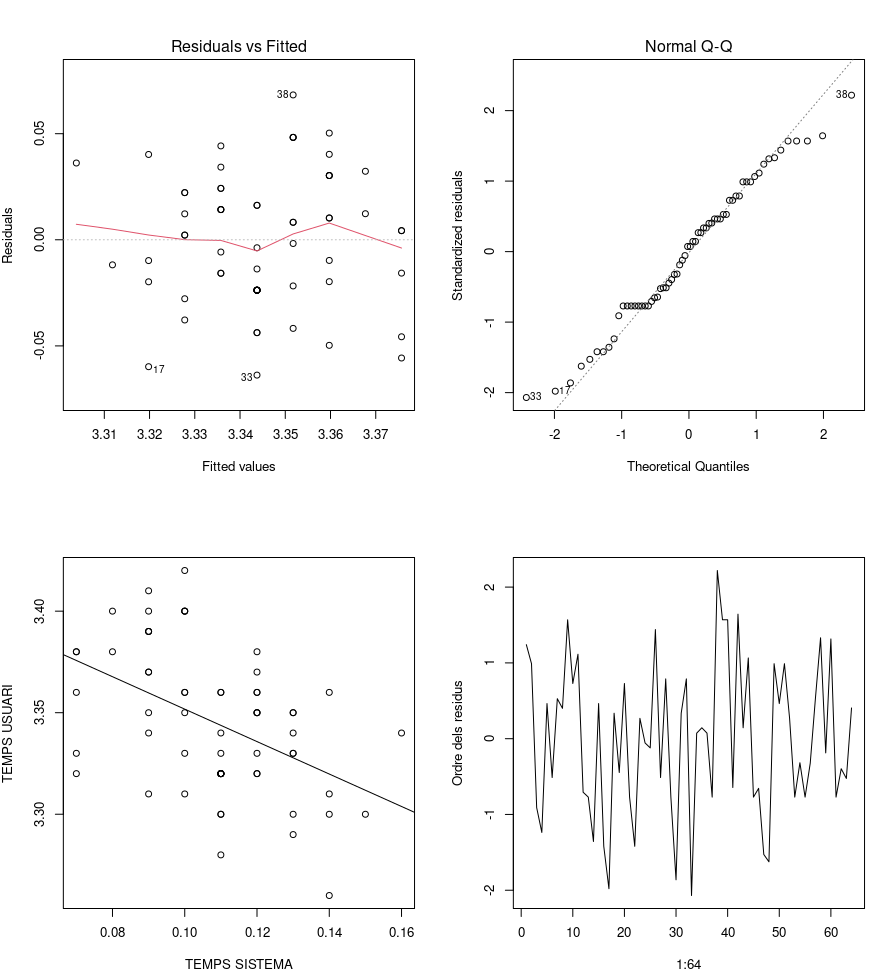
\includegraphics[width=15cm, height=10cm]{prem3.png}
  \caption{Premisses}
  \label{fig:prem3}
\end{figure} 

Igual que abans, tot i que són poques dades, res s'oposa a validar cap de les 4 premisses.
\hfill \break
Ara, podem usar la comanda lm per poder veure com és la recta a la que s'ajusten el temps d'usuari i de sistema al programa d'ordenació
de vectors, per poder inferir quin tipus de relació hi ha entre ells:

\begin{figure}[h!]
  \centering
  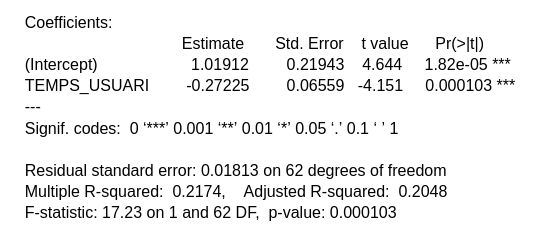
\includegraphics[width=10cm, height=6cm]{lm3.png}
  \caption{Sortida comanda lm}
  \label{fig:lm3}
\end{figure} 

A la Figura \ref{fig:lm3} es pot veure com l'R-squared ara és més gran, de 0.2174, però tot i així continua essent petit. És a dir, a la
partida d'EDA el temps de sistema determina una mica més la variabilitat del temps d'usuari, pero continua sent poc. Per tant, per segon cop,
no té sentit analitzar la recta que ens proporciona la comanda d'R.

\section{Discussió dels resultats}
\subsection{Conclusió}
Pel que fa a la mitjana del temps total que tarden les shells en realitzar totes les execucions, els resultats obtinguts ens mostren com hi ha una shell la mitjana 
de la qual hem inferit és menor a les demés: Zshell. Tot i així, com que s'obtenen diferències entre shells amb uns p-values superiors al risc (sota l'hipòtesi que la
diferència és 0), llavors les podem considerar igual de ràpides. No hi ha res que s'oposi a dir que són igual de ràpides, almenys amb les dades que hem recollit. De fet, en el 
nostre cas, els temps entre programes són més diferents que entre shells. En conclusió, les dades mostren que no hi ha diferències entre les shells, més enllà que una d'elles
tingui la mitjana mínima, però no significativament inferior a les altres. \break

Per altra banda, en quant a la relació entre el temps d'usuari i el temps de sistema, els resultats ens diuen que el temps de sistema no determina la variabilitat 
del temps d'usuari, en cap dels dos programes que hem usat. Aquesta conclusió resulta tenir molt de sentit, ja que en l'execució del programa de gestió de processos, que 
al final vam decidir no incloure pel que s'explicarà a l'apartat posterior, es veia com els temps de sistema eren superiors als temps d'usuari, cosa totalment inversa al que 
s'obté a l'ordenació de vectors i a la partida d'EDA.

És a dir, en relació a les hipòtesis que teníem inicialment, que la diferència de velocitat entre les shells era nul·la i que no hi havia relació lineal entre el temps de sistema
i el temps d'usuari, podem dir que eren certes.

\subsection{Limitacions i problemes trobats}
La major limitació del nostre estudi ve donada pel reduït nombre d'execucions realitzades i el fet de no tenir en compte una amplia variabilitat de programes, per poder assegurar
encara més la "justicia" a l'hora de comparar les shells. Una possible millora a realitzar seria fer un únic programa que faci moltes coses diferents i realitzar moltes execucions
d'aquest programa a cadascuna de les shells.

Pel que fa als problemes trobats, com s'havia mencionat anteriorment, inicialment voliem realitzar, per cada shell, quatre execucions de quatre programes diferents,
els dos que s'usen en aquest treball i uns altres dos:
\begin{itemize}
  \item tree /: \emph{tree} es tracta d'una comanda UNIX que s'usa per llistar de forma recursiva el contingut d'un directori. Llavors, si fem tree /, per ser / el directori
    arrel del sistema operatiu, es llistaria tot el contingut del sistema de fichers.
  \item Gestió de processos: disposàvem d'un altre programa en bash script on el procés pare crea 1000 processos fills que passen a calcular i mostrar per sortida estàndard 
    el nombre de fibonacci amb índex 40. Després d'això el pare espera a la mort dels fills mitjançant la crida a sistema wait per eliminar la seva informació de les 
    estructures de dades del kernel.
\end{itemize} 
L'objectiu que teniem a l'usar aquests altres dos programes era que hi hagués més variabilitat en quant a programes, per no afavorir a una shell que sigui millor en una gestió 
concreta. Però ens vam trobar amb un greu problema a l'hora de voler fer l'anàlisi del temps total d'execució per part de cada shell: la premissa de normalitat no es complia. Això
era degut a que, com que la diferència entre els temps dels dos programes que usem en el treball i aquest altres dos era molt diferent, i s'observaben tres subconjunts molt diferents 
a les gràfiques. Una opció podria haver sigut analitzar els temps associat a cada subconjunt de programes, però vam preferir prescindir d'aquests dos i realitzar més execucions
de la partida d'EDA i l'ordenació de vectors per donar més fiabilitat a l'estudi. De totes, formes, tant la recollida de dades qua vam fer inicialment com el programa de gestió
de processos estaran disponibles a \nameref{ANNEX}.

\subsection{Treballs futurs}
Com a proposta de treball futur, es podria fer el que s'ha comentat abans, comparar les shells fent un únic programa amb molta variabilitat de còmput, i realitzar moltes
execucions d'aquest a cada shell. També es podrien evaluar shells que no s'han contemplat en aquest treball i fins i tot analitzar el seu rendiment en funció de l'arquitectura
del computador, o qualsevol altre aspecte que pugui afectar al temps que tarda cada shell.

\newpage
\section*{ANNEX}

\label{ANNEX}

A continuació es pot observar el codi en bashscript del programa que ordena un vector de 10000 elements. El vector,
com s'ha dit anteriorment, és sempre el mateix i de fet es troba present al codi font, però no l'inclourem en aquest
document per motius obvis.
\begin{lstlisting}[language=Bash, caption="Programa en bashscript: Ordenació d'un vector de 10000 elements"]
  #!/bin/bash

  function partition {
    let i=$2-1
    let pivot=${x[$3]}
  
   for(( j="$2"; j<"$3"; j++ ))
    do
      if [ "${x[$j]}" -lt "$pivot" ]
      then
        let i=i+1
        let temp=${x[$i]}
        x[$i]=${x[$j]}
        x[$j]=$temp
      fi
    done

    let temp=${x[$((i+1))]}
    x[$((i+1))]=${x[$3]}
    x[$3]=$temp
  
    k=$((i+1))
  }

  function quicksort {
    if [ "$2" -lt "$3" ]
    then
      partition x $2 $3   
      let pi=k
      quicksort x $2 $((pi-1))
      quicksort x $((pi+1)) $3
    fi 
  }
  echo -n "Sorted array: "
  for i in "${x[@]}"
  do
    echo -n "$i "
  done
  echo
\end{lstlisting}

\newpage

Aquí podem veure el codi en bashscript del programa que crea 1000 processos que calculen i mostren per sortida estàndard 
el nombre de fibonacci amb índex 40:

\begin{lstlisting}[language=Bash, caption="Programa en bashscript: Gestió de processos"]
  #!/bin/bash
  
  fibonacci() {
    local n=$1
    local a=0
    local b=1
    for ((i=0; i<n; i++)); do
      local c=$((a + b))
      a=$b
      b=$c
    done
    echo $a
  }

  for ((i=1;i<=1000;i++)); do
    (
      echo "Proceso $i: $(fibonacci 5000)"
    ) &
  done

  wait

\end{lstlisting} 

\vspace{5mm} %5mm vertical space
Finalment, a través d'aquest enllaç es pot accedir a un repositori de GitHub on es pot veure tot el codi del jugador PEplayer
per les partides d'EDA, a més del ficher .xlsx amb totes les dades que hem usat i les comandes de R emprades:
\url{https://github.com/Isma1108/Shell_mes_rapida}
\end{document}
